% This is a simple template for an iSIM LaTeX lab using the "article" class. Read both the text and the comments--everything is useful!

\documentclass[11pt]{article} % use larger type; default would be 10pt

% There's a lot of boilerplate crap that you don't need to understand
\usepackage[utf8]{inputenc}

% These are packages you may need... It doesn't cost anything to include them all, so you might as well.
\usepackage{amstext} %allows you to put text in math mode
\usepackage{amsmath} %includes lots of math-related capabilities
\usepackage{graphicx} %allows you to include pictures
\usepackage{float} %improves the use of floating objects (like picutes)
\usepackage{caption} %allows you to change caption styles on figures
\usepackage{epstopdf} %automatically converts EPS files (like from matlab)
\usepackage{hyperref} %allows you to include links
\usepackage{varioref} %requirement of fancyref
\usepackage{fancyref} %allows really nice looking and convienient references
\usepackage[section]{placeins} %makes your figures not float past section barriers
\usepackage{perpage} %restarts footnote numbering by page
\usepackage[margin=1in, paperwidth=8.5in, paperheight=11in]{geometry} %I'll bet you can figure this one out
\MakeSorted{figure} %deals with figures using both [h] and [H]

% Makes sure your document compiles when you screw up the references
\vrefwarning

% Uncomment the following line to default all of your figures to [H] (explained later)
%\float­place­ment{fig­ure}{H}

%add some metadata to the PDF produced
 % \pdfinfo{/Author (Eric Miller)

%%% The "real" document content comes below...

\title{Lab Report: Glucose monitor}
\author{Eric Miller}
%\date{Now} % Leave this commented to automatically display the current date. Otherwise, you can redefine it here.

\begin{document}
\maketitle % Make sure to include this (after begin{document}, or you'll have no title!

%\begin{abstract}
%\LaTeX~is a markup language (like HTML) that allows you to create beautiful lab reports (among other things) with a wide variety of STEM-oriented features. Like almost everything else, you can find out a lot about using \LaTeX~by using Google. You can also have a look at the wikibook\footnote{You can add links like so: \href{http://en.wikibooks.org/wiki/LaTeX}{\LaTeX~Wikibook} Have a look at that wikibook--it contains almost everything you'll ever need to know about \LaTeX.} which is usually among the first few Google results for most \LaTeX-related queries.
%\end{abstract}

\section{Voltage Source}

Having my younger siblings visiting for Family Weekend, I asked them to find a pair of resistors ending in "k" with a ratio of approximately $2:3$. The resulting resistor values were nominally $4 k\Omega$ and $6.04 k\Omega$, for a theoretical voltage divider output of 
$$5V*\frac {4 k\Omega} {4 k\Omega + 6.04 k\Omega} = 1.992 V$$

The actual measured value was slightly lower, at $1.97V$, but the difference wasn't significant enough to be a problem.

%Note the use of \Fref here... This automatically creates a reference to your figure, no matter where it is in the document. If it is on a different page, \Fref will include the page of the figure. For this to work, you have to provide intelligent labels, i.e. fig:whatever for figures. Labels should be lowercase and have no spaces.	

%the [!ht] here means "LaTeX, I would very much like you to put this figure here, but if you can't that's ok, just make sure it's at the top of some other page"
% However, because you (what a smart cookie you are) decided to include the float package, you can use the option [H], which tells LaTeX "PUT THE ****ing FIGURE HERE OR I WILL GO BACK TO USING WORD YOU GODDAMN STUPID PIECE OF **** TYPESETTING PROGRAM" 
\begin{figure}[H]
	\centering
	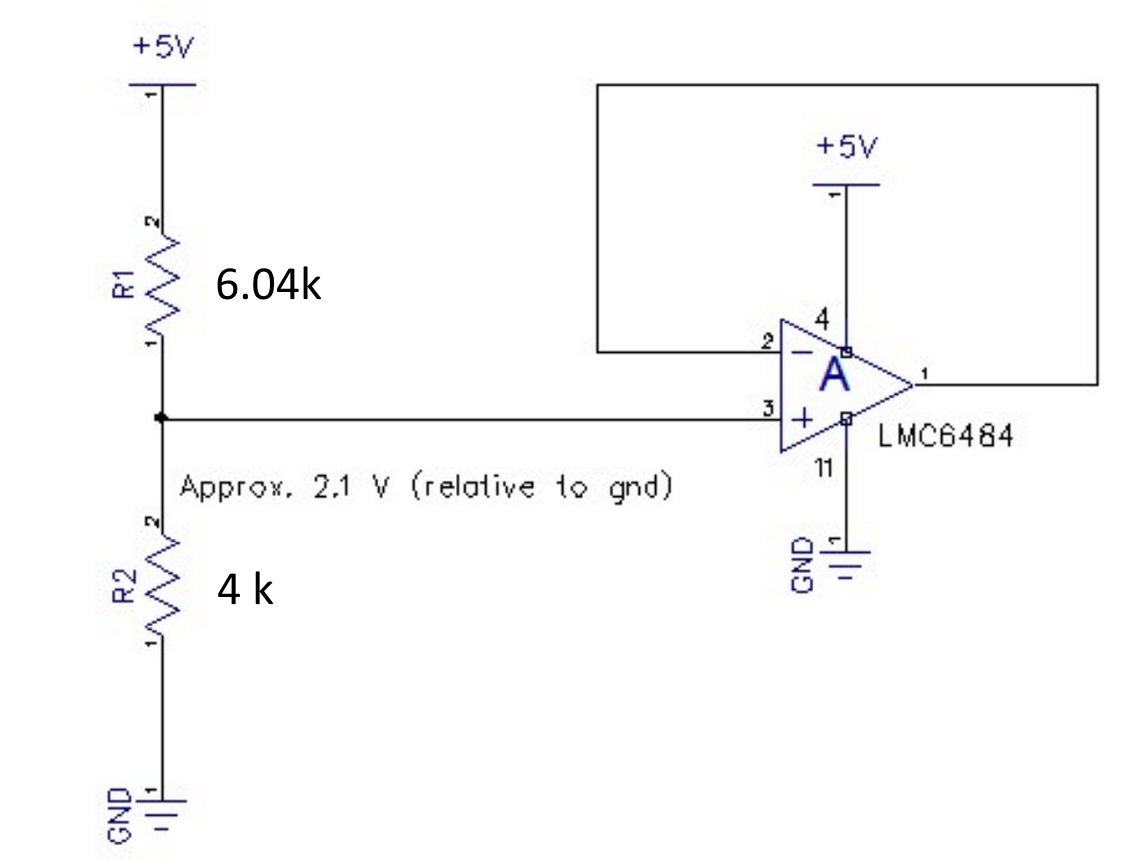
\includegraphics[width=.8\textwidth]{CD1.png}
	\caption{Voltage Divider circuit}
\end{figure}

\begin{figure}[H]
	\centering
	%instead of entering the width in terms of textwidth, you can use a set number of inches, or pt, or mm, or whatever
	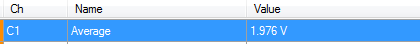
\includegraphics[width=.5\textwidth]{VoltageDivider.png}
	%Make sure to caption your figures! LaTeX will automatically number them for you.
	\caption{Voltage Divider results}
 	\label{fig:awesome}
\end{figure}

%You can make subsections (and subsubsections) if you need to go into detail
\section{Measure Resistance}




\end{document}
